\definecolor{rpisecbgcolor}{RGB}{21, 24, 32} % 151820
\definecolor{cybercyan}{RGB}{42, 171, 219} % 2aabdb
\definecolor{cybergreen}{RGB}{106, 220, 169} % 6adca9
\definecolor{cyberpink}{RGB}{248, 106, 140} % f86a8c

\setbeamercolor{normal text}{fg=white}
\setbeamercolor{frametitle}{fg=cybercyan}
\setbeamercolor{title}{fg=cybercyan}
\setbeamercolor{structure}{fg=cybercyan}

%>>> [0x15,0x18,0x20]
%[21, 24, 32]
% convert rpisec_background.png -alpha set -fill '#15182080' -draw 'rectangle 0 0 1090 1216' rpisec_background2.png
% convert probable_prime.png -alpha set -fill '#151820c0' -draw 'rectangle 0 0 414 836' probable_prime2.png
\usebackgroundtemplate{
\colorbox{rpisecbgcolor}{\raisebox{1pt}[\paperheight][\depth]{\hspace{0.6\paperwidth}
%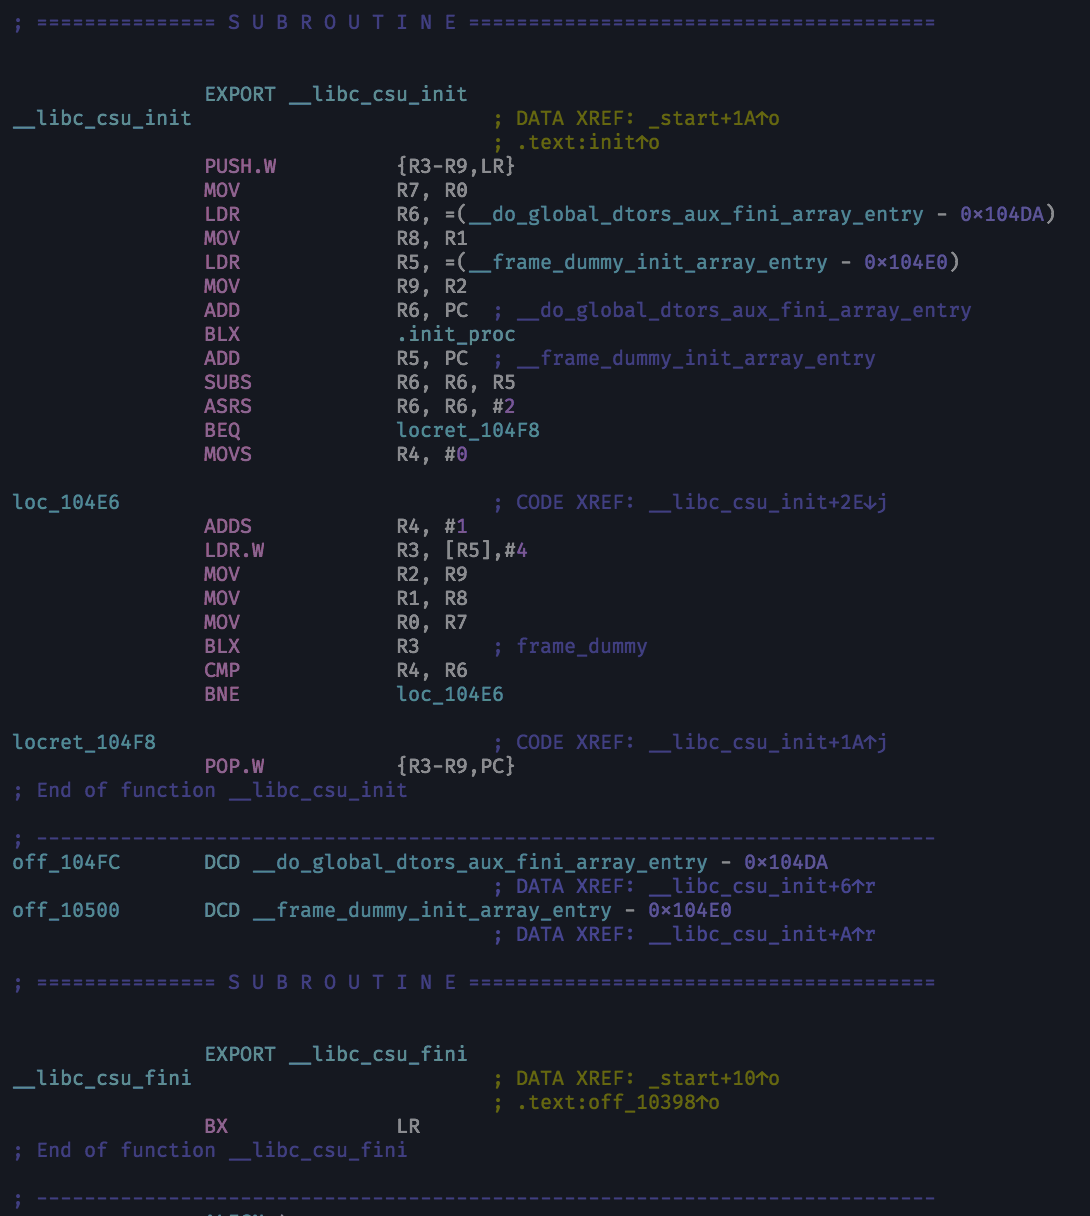
\includegraphics[width=0.4\paperwidth, height=\paperheight]{rpisec_background2.png}
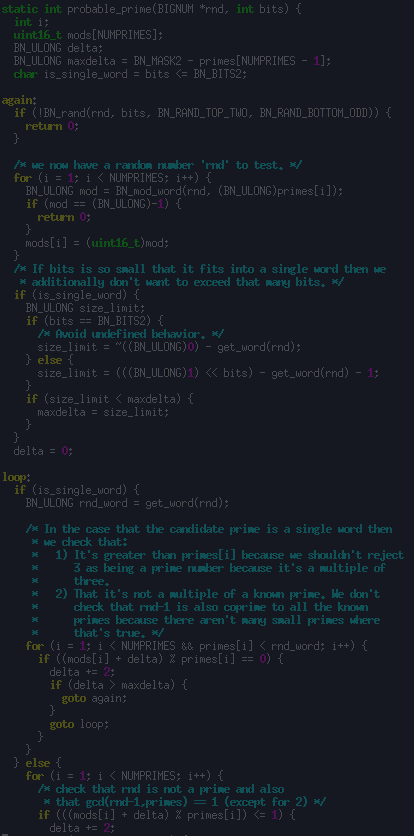
\includegraphics[width=0.4\paperwidth, height=\paperheight]{../rsa_2019_10_29/probable_prime2.png}
}}
}

\newcommand{\SlideWithCenteredText}[1]{
  \begin{frame}
  \vfill
  \centering
  \begin{beamercolorbox}[sep=8pt,center,shadow=true,rounded=true]{title}
    \usebeamerfont{title}#1\par%
  \end{beamercolorbox}
  \vfill
  \end{frame}
}

\newcommand{\questionsslide}[1]{\SlideWithCenteredText{Any questions#1?}}

% https://tex.stackexchange.com/questions/178800/creating-sections-each-with-title-pages-in-beamers-slides
\AtBeginSection[]{
\SlideWithCenteredText{\insertsectionhead}
}

